\documentclass[xcolor=table,dvipsnames,svgnames,aspectratio=169,fontset=fandol]{ctexbeamer}
% 可以通过 fontset=macnew / fontset=ubuntu / fontset=windows 选项切换字体集
% 如果ubuntu字体集无法使用,可以尝试fandol
\usepackage{tikz}
\usepackage[normalem]{ulem}
\usetikzlibrary{arrows}
\usepackage{amsmath}
\usepackage{mflogo}
\usepackage{graphicx}
\usepackage{ccicons}
\usepackage{hologo}
\usepackage{colortbl}
\usepackage{shapepar}
\usepackage{hyperxmp}
\usepackage{booktabs}
\usepackage{qrcode}
\usepackage{listings}
\usepackage{tipa}
\usepackage{multicol}
\usepackage{datetime2}
\usepackage{fontawesome5}
\usepackage{hyperref}
\usepackage{enumitem}
\usepackage{bm}
\usepackage[backend=biber,style=gb7714-2015]{biblatex}
\addbibresource{thesis.bib}
\graphicspath{{figures/}}
\hypersetup{
  pdfsubject = {上海交通大学图书馆专题培训讲座},
  pdfauthor = {Alexara Wu},
  pdfcopyright = {Licensed under CC-BY-SA 4.0. Some rights reserved.},
  pdflicenseurl = {http://creativecommons.org/licenses/by-sa/4.0/},
  unicode = true,
  psdextra = true,
  pdfdisplaydoctitle = true
}

\DeclareOptionBeamer{en}

\pdfstringdefDisableCommands{
  \let\\\relax
  \let\quad\relax
  \let\hspace\@gobble
}
\renewcommand{\TeX}{\hologo{TeX}}
\renewcommand{\LaTeX}{\hologo{LaTeX}}
\newcommand{\BibTeX}{\hologo{BibTeX}}
\newcommand{\XeTeX}{\hologo{XeTeX}}
\newcommand{\pdfTeX}{\hologo{pdfTeX}}
\newcommand{\LuaTeX}{\hologo{LuaTeX}}
\newcommand{\MiKTeX}{\hologo{MiKTeX}}
\newcommand{\MacTeX}{Mac\hologo{TeX}}
\newcommand{\beamer}{\textsc{beamer}}
\newcommand{\XeLaTeX}{\hologo{Xe}\kern-.13em\LaTeX{}}
\newcommand{\pdfLaTeX}{pdf\LaTeX{}}
\newcommand{\LuaLaTeX}{Lua\LaTeX{}}
\def\TeXLive{\TeX{} Live}
\let\TL=\TeXLive
\newcommand{\SJTUThesis}{\textsc{SJTUThesis}}
\newcommand{\SJTUThesisVersion}{1.1.0}
\newcommand{\SJTUThesisDate}{2023/3/24}
\newcommand{\SJTUBeamer}{\textsc{SJTUBeamer}}
\newcommand{\SJTUBeamerVersion}{3.0.0}
\newcommand{\SJTUBeamerDate}{2022/11/22}
\newcommand\link[1]{\href{#1}{\faLink}}
\newcommand\pkg[1]{\texttt{#1}}
\def\cmd#1{\texttt{\color{structure}\footnotesize $\backslash$#1}}
\def\env#1{\texttt{\color{structure}\footnotesize #1}}
\def\cmdxmp#1#2#3{\small{\texttt{\color{structure}$\backslash$#1}\{#2\}
\hspace{1em}\\ $\Rightarrow$\hspace{1em} {#3}\par\vskip1em}}
\lstset{
  language=[LaTeX]TeX,
  basicstyle=\ttfamily\footnotesize,
  tabsize=2,
  keywordstyle=\bfseries\ttfamily\color{cprimary},
  commentstyle=\sl\ttfamily\color[RGB]{100,100,100},
  stringstyle=\ttfamily\color[RGB]{50,50,50},
  extendedchars=true,
  breaklines=true,
}

\usetheme[maxplus,blue,smoothbars]{sjtubeamer}
% 使用 maxplus/max/min 切换标题页样式
% 使用 red/blue 切换主色调
% 使用 light/dark 切换亮/暗色模式
% 使用外样式关键词以获得不同的边栏样式
%   miniframes infolines  sidebar
%   default    smoothbars split	 
%   shadow     tree       smoothtree
% 使用 topright/bottomright 切换徽标位置
% 使用逗号分隔列表以同时使用多种选项

\author{侯力广  521070910043}
\date{\the\year \,.\the\month \,}
%\subject{LaTeX, 论文排版, SJTUThesis}
\title[Dynamics of Cognition]
{\textbf{Dynamics of Decision Making}} 

\setbeamercolor{block title alerted}{use=structure,fg=white,bg=structure.fg!88!black}
\setbeamercolor{block body alerted}{parent=normal text,use=block title,bg=block title.bg!10!white}


%=================================================================
%==================================================================

\begin{document}

\maketitle
%-----------------------------------------------------------------------

\begin{frame}{Introduction}
  We make multiple decisions in daily life. (Examples...)
  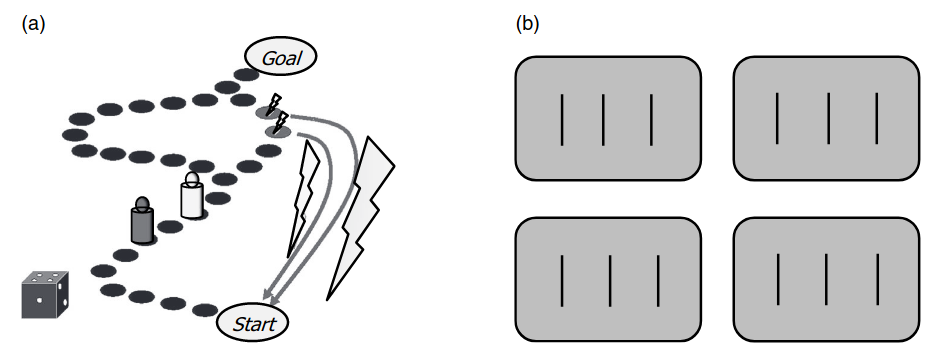
\includegraphics[width=0.75\textwidth,height=0.6\textheight]{decision_examples.png}
    
  $\qquad\qquad$Board games \footnote{\scalebox{0.8}{Platt ML, Huettel SA. \textit{Risky business: the neuroeconomics of decision making under uncertainty.} Nat Neurosci. 2008 Apr }}  $\qquad\qquad$ Perceptual decision making
\end{frame}

\begin{frame}{Introduction}
  Generally, decision making requires:\footnote{\scalebox{0.8}{Rangel et all. \textit{ A framework for studying the neurobiology of value-based decision making.} Nat Rev Neurosci. 2008}}
  \begin{itemize}
    \item 1. a suitable \textbf{representation} of inputs and potential outcomes as well as of the values attached to the options
    \item 2. a \textbf{selection} process that picks one of the options
    \item 3. potentially also some \textbf{feedback} that enables learning so as to achieve improved performance over several trials 
  \end{itemize}
  Here, we focus on the dynamic selection between different options in the context of perceptual decision making, driven by the convenience of measuring neuronal activity.
\end{frame}

%\begin{frame}{Introduction}
%  The aim of this report is not to review the field of cognitive science, but rather to show by way of an example how models of neuronal activity can be linked to fundamental questions of cognition.
%  \vskip 12pt
%  The Hodgkin–Huxley model describes the generation of action potentials on the level of ion channels and ion current flow. It is the starting point for detailed biophysical neuron models
%\end{frame}

%-----------------------------------------------------------------------

\begin{frame}{Contents}
  \tableofcontents[hideallsubsections]
\end{frame}

%
%-----------------------------------------------------------------------

\section{Perceptual decision making}

%\footnote{\scalebox{0.8}{Gold JI, Shadlen MN. \textit{ The neural basis of decision making. } Annu Rev Neurosci. 2007}}
%
\begin{frame}{Perceptual decision making}
  A classical study of perceptual decision making in monkeys \footnote{\scalebox{0.8}{Salzman et al.\textit{ Cortical microstimulation influences perceptual judgements of motion direction.} Nature. 1990}}
  
  \begin{center}
  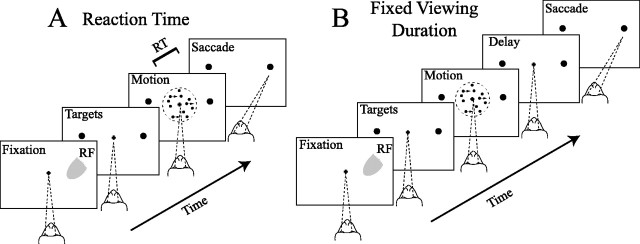
\includegraphics[width=0.6\textwidth,height=0.4\textheight]{monkey.png}
  \end{center}

  The stimulus consists of a random pattern of moving dots, where most of the dots move coherently in the same direction. The monkey has been trained to indicate the perceived motion direction by saccadic eye movements to one of two targets.
\end{frame}

\begin{frame}{Perceptual decision making}
  \begin{columns}
    \column{0.7\linewidth}
    \textbf{Biologists have found that:}

    \vskip 8pt
    Different neurons in the middle temporal visual area (MT) respond to different directions of motion, and clusters of neighboring neurons share receptive fields with a similar preferred direction of motion. 

    \column{0.3\linewidth}
    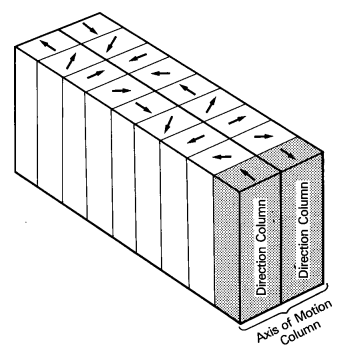
\includegraphics[width=0.8\textwidth,height=0.65\textheight]{mt.png}
  \end{columns}\footnote{\scalebox{0.8}{Albright et al. \textit{Columnar organization of directionally selective cells in visual area MT of the macaque} J Neurophysiol. 1984}}
\end{frame}

\begin{frame}{Perceptual decision making}

  The location of the receptive field and the preferred direction of motion is determined by varying the movement angle and the location of the random dot stimulus. Once the receptive properties of the local MT neurons have been determined, only two different classes of stimuli are used.\footnote{\scalebox{0.8}{Salzman et al.\textit{ Cortical microstimulation influences perceptual judgements of motion direction.} Nature. 1990}}
  \begin{center}
    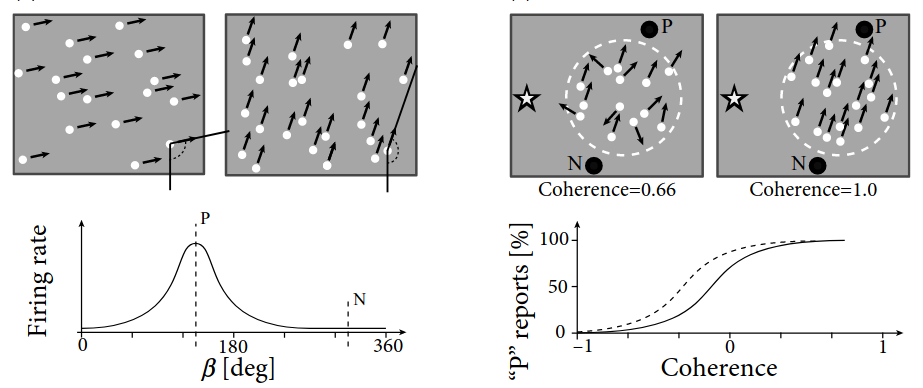
\includegraphics[width=0.65\textwidth,height=0.45\textheight]{monkey2.png}
  \end{center}
\end{frame}

\begin{frame}{Perceptual decision making}

  \textbf{Conclusion:} the perceptual decision of the monkey relies on the motion information represented in the activity of MT neurons.\footnote{\scalebox{0.8}{Salzman et al.\textit{ Cortical microstimulation influences perceptual judgements of motion direction.} Nature. 1990}} 

  \vskip 12pt

  \textbf{After that:} neuroscientists have continuously conducted such monkey perceptual decision making experiments, leading to many new discoveries\footnote{\scalebox{0.8}{Roitman et al.\textit{ Response of neurons in the lateral intraparietal area during a combined visual discrimination reaction time task.}2002}} \footnote{\scalebox{0.8}{Rangel et all. \textit{ A framework for studying the neurobiology of value-based decision making.} Nat Rev Neurosci. 2008}}, including the modeling of decision making.

\end{frame}
%-----------------------------------------------------------------------

\section{Competition through common inhibition}

\begin{frame}{Competition through common inhibition}
  The essential features of the experiments of Roitman and Shadlen (2002) can be described by a simple model of decision making where two excitatory populations compete with each other through a shared inhibitory population. \footnote{\scalebox{0.8}{Wang etal.\textit{Anatomical,physiological,molecular and circuit properties of nest basket cells in the developing somatosensory cortex.}2002}}  
  \begin{columns}
    \column{0.5\linewidth}
    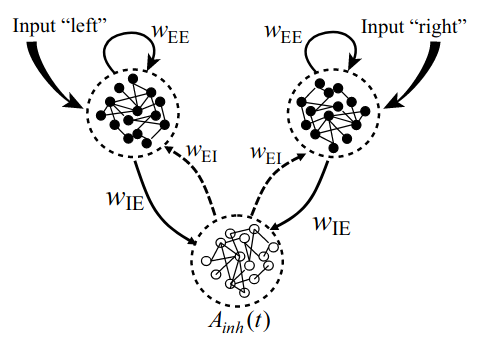
\includegraphics[width=0.9\textwidth,height=0.6\textheight]{competition.png}
    \column{0.5\linewidth}
    \textbf{Note:} Input "left" brings excitatory population 1 activity $A_{E,1}(t)$. Each excitatory population has connection weights $w_{EE}$. The inhibitory population receives input of strength $w_{IE}$ from the two excitatory populations and sends back inhibition of strength $w_{EI}$.
  \end{columns}
\end{frame}


\begin{frame}{Competition through common inhibition}
  The input into each population is described as a mean plus some noise.

  The following picture shows presentations of an unbiased stimulus, where the input to the left and right populations has an equal mean but different realizations of noise. \footnote{\scalebox{0.8}{Wang etal.\textit{Anatomical,physiological,molecular and circuit properties of nest basket cells in the developing somatosensory cortex.}2002}}   
  \begin{center}
  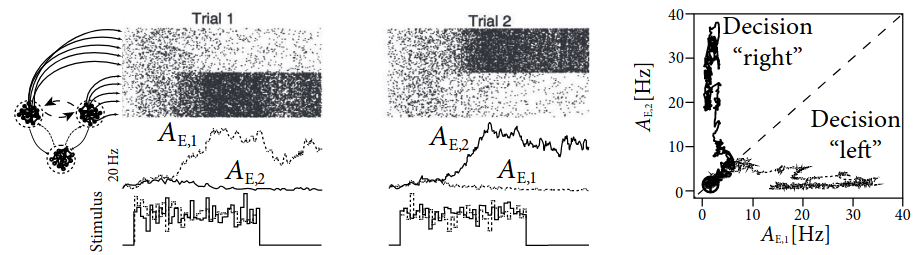
\includegraphics[width=0.8\textwidth,height=0.4\textheight]{competition2.png}
  \end{center}

  \vskip -8pt
  In the absence of stimulation, the activity of both excitatory populations exhibits a low firing rate of less than 5 Hz (circle). Upon stimulation, the dynamics converge.

\end{frame}


%-----------------------------------------------------------------------

\section{Dynamics of decision making}

\begin{frame}{Dynamics of decision making}

  \textbf{Next,} we will present a mathematical analysis of decision-making in models of interacting populations, divided into the following four parts.

    \begin{itemize}
      \item \textbf{P1.} Give the rate equations for a model with three populations, two excitatory ones which interact with a common inhibitory population. 
      \item \textbf{P2.} Reduce the rate model with three populations to a simplified system described by two differential equations.
      \item \textbf{P3.} Analysis the fixed points of the two-dimensional dynamical system in the phase plane for several situations relevant to experiments on decision making.
      \item \textbf{P4.} Generalize the formalism of competition through shared inhibition to the case of K competing populations.
    \end{itemize}

\end{frame}

\begin{frame}{P1. Model with three populations}
\textbf{1. About rate models:}

\vskip 5pt
Let $A(t)$ represent the average firing rate of a population of homogeneous neurons, and let the input potential be denoted as $h(t)$. Let $F$ be the gain function, then the population activity can be expressed as:\footnote{\scalebox{0.8}{Wulfram Gerstner, Werner M. Kistler, Richard Naud, Liam Paninski.\textit{Neuronal Dynamics} Cambridge University Press. 2014}}   

$$A(t)=F(h(t)).$$

We use an exponential kernel to perform convolution to represent $h(t)$:

$$h(t)=\frac{R}{\tau_m}\int_{0}^{\infty}e^{-\frac{s}{\tau_m}}I(t-s)ds,$$

where $\tau_m$ is the membrane time constant and $R$ is the membrane resistance.
\end{frame}

\begin{frame}{P1. Model with three populations}
  By applying integration by parts, the above expression is equivalent to the equation

  $$\tau_m\frac{dh(t)}{dt}=-h+RI(t),$$

  Therefore, the general form of the rate model is:\footnote{\scalebox{0.8}{Wulfram Gerstner, Werner M. Kistler, Richard Naud, Liam Paninski.\textit{Neuronal Dynamics} Cambridge University Press. 2014}}   

  \begin{equation}
    \begin{aligned}
      A(t)&=F(h(t))\\
      \tau_m\frac{dh(t)}{dt}&=-h+RI(t)
    \end{aligned}
  \end{equation}

\end{frame}

\begin{frame}{P1. Model with three populations}
  \textbf{2. Rate model with three populations:}

  \vskip 5pt
  Let $g_E$ and $g_{inh}$ be the gain functions of excitatory and inhibitory neurons respectively.

  \begin{equation}
    \begin{aligned}
      A_{E,1}&=g_E (h_{E,1})\\
      A_{E,2}&=g_E (h_{E,2})\\
      A_{inh}&=g_{inh} (h_{inh})\\
      \tau_E \frac{dh_{E,1}}{dt}&=-h_{E,1}+w_{EE}g_E (h_{E,1})+w_{EI}g_{inh} (h_{inh})+RI_1\\
      \tau_E \frac{dh_{E,2}}{dt}&=-h_{E,2}+w_{EE}g_E (h_{E,2})+w_{EI}g_{inh} (h_{inh})+RI_2\\
      \tau_{inh} \frac{dh_{inh}}{dt}&=-h_{inh}+w_{IE}g_E (h_{E,1})+w_{IE}g_{E} (h_{E,2})
    \end{aligned}
  \end{equation}

\end{frame}

\begin{frame}{P2. Effective inhibition}
  The system of three populations is still complex. To reduce it to two dimensions and utilize phase plane analysis tools, we make the following assumptions.

  \vskip 5pt
\textbf{Assumption 1.}

\vskip 5pt
The membrane time constant $\tau_{inh} \ll \tau_{E}$, i.e. we consider the limit of a separation of time scales $\tau_{inh} \ll \tau_{E}\rightarrow 0$. Therefore we can treat the dynamics of $h_{inh}$ in as instantaneous, so that the inhibitory potential is always at its fixed point

$$h_{inh}=w_{IE}[g_E (h_{E,1})+g_E (h_{E,2})]$$

According to the expression of the convolution kernel, such an assumption implies that the current decay in the excitatory neuron population is slower than that in the inhibitory neuron population, which is consistent with the fact that excitatory synapses typically possess \textbf{NMDA receptors}.

\end{frame}

\begin{frame}{P2. Effective inhibition}

  After assuming the separation of time scales between inhibition and excitation, the dynamical equations for $h_{E,1}$ and $h_{E,2}$ become:

  \begin{equation*}
    \begin{aligned}
      \tau_E \frac{dh_{E,1}}{dt}&=-h_{E,1}+w_{EE}g_E (h_{E,1})+w_{EI}g_{inh} (w_{IE}[g_E (h_{E,1})+g_E (h_{E,2})])+RI_1\\
      \tau_E \frac{dh_{E,2}}{dt}&=-h_{E,2}+w_{EE}g_E (h_{E,2})+w_{EI}g_{inh} (w_{IE}[g_E (h_{E,1})+g_E (h_{E,2})])+RI_2
    \end{aligned}
  \end{equation*}

\end{frame}

\begin{frame}{P2. Effective inhibition}

  \textbf{Assumption 2.}

  \vskip 5pt
  The second assumption is not absolutely necessary, but it makes the remaining two equations more transparent. We assume a linear gain function
  $$g_{inh}(h_{inh})=\gamma h_{inh}$$

  with a slope factor $\gamma>0$. Then equations for $h_{E,1}$ and $h_{E,2}$ become:

  \begin{equation}
    \begin{aligned}
      \tau_E \frac{dh_{E,1}}{dt}&=-h_{E,1}+(w_{EE}-\alpha)g_E (h_{E,1})-\alpha g_E (h_{E,2})+RI_1\\
      \tau_E \frac{dh_{E,2}}{dt}&=-h_{E,2}+(w_{EE}-\alpha)g_E (h_{E,2})-\alpha g_E (h_{E,1})+RI_2
    \end{aligned}
  \end{equation}

  where we have introduced a parameter $\alpha=-\gamma w_{EI}w_{IE}>0$.

\end{frame}

\begin{frame}{P2. Effective inhibition}
  \textbf{Thus,} the model of three populations has been replaced by a model with two excitatory populations that interact with an effective inhibitory coupling of strength $\alpha$.

  \vskip 5pt
  \begin{columns}
    \column{0.5\linewidth}
    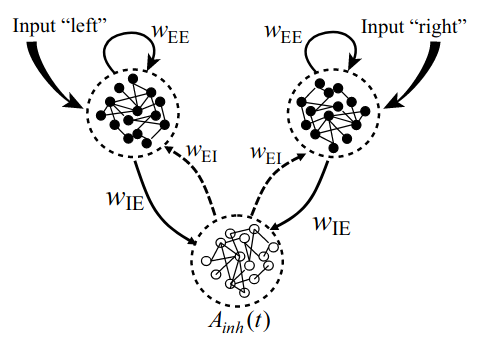
\includegraphics[width=0.9\textwidth,height=0.6\textheight]{competition.png}
    \column{0.5\linewidth}
    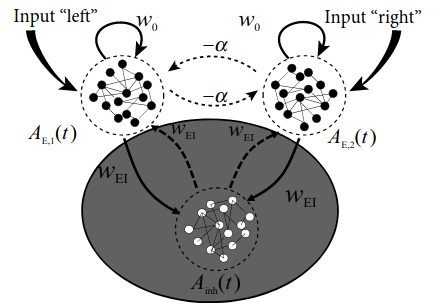
\includegraphics[width=0.85\textwidth,height=0.6\textheight]{competition3.png}
  \end{columns}
\end{frame}

\begin{frame}{P3. Phase plane analysis}
  \begin{columns}
    \column{0.5\linewidth}
    \textbf{$I_1=I_2=0$}:

    \vskip 12pt
    There exists only a single fixed point $h_{E,1} = h_{E,2} \thickapprox  0$, corresponding to a small level of spontaneous activity.
    \column{0.5\linewidth}
    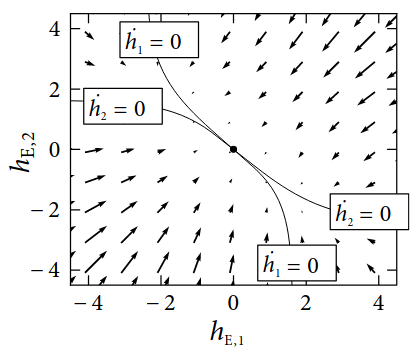
\includegraphics[width=0.9\textwidth,height=0.8\textheight]{phase1.png}
  \end{columns}\footnote{\scalebox{0.8}{Wulfram Gerstner, Werner M. Kistler, Richard Naud, Liam Paninski.\textit{Neuronal Dynamics} Cambridge University Press. 2014}}   
\end{frame}

\begin{frame}{P3. Phase plane analysis}
  \begin{columns}
    \column{0.5\linewidth}
    \textbf{$I_1 > 0 = I_2$}:

    \vskip 12pt
    The fixed point moves to an asymmetric position where population 1 exhibits much stronger activity than population 2. 

    \column{0.5\linewidth}
    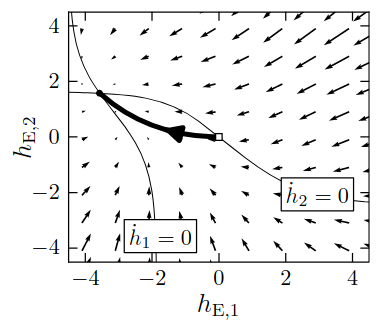
\includegraphics[width=0.9\textwidth,height=0.8\textheight]{phase2.png}
  \end{columns}\footnote{\scalebox{0.8}{Wulfram Gerstner, Werner M. Kistler, Richard Naud, Liam Paninski.\textit{Neuronal Dynamics} Cambridge University Press. 2014}}   
\end{frame}

\begin{frame}{P3. Phase plane analysis}
  \begin{columns}
    \column{0.5\linewidth}
    \textbf{$I_1=I_2>0$}:

    \vskip 12pt
    Three fixed points exist and the symmetric one is a saddle point. The two other fixed points occur at equivalent positions symmetrically to the left and right of the diagonal.
    \column{0.5\linewidth}
    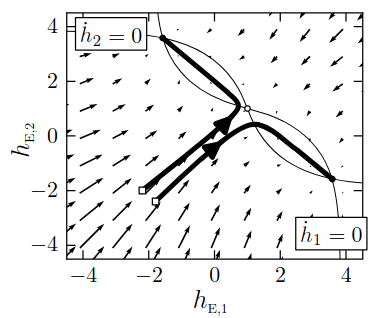
\includegraphics[width=0.9\textwidth,height=0.8\textheight]{phase3.png}
  \end{columns}\footnote{\scalebox{0.8}{Wulfram Gerstner, Werner M. Kistler, Richard Naud, Liam Paninski.\textit{Neuronal Dynamics} Cambridge University Press. 2014}}   
\end{frame}

\begin{frame}{P3. Phase plane analysis}
  Decisions correspond to a ball rolling down an energy landscape, plotted as a function of a formal decision variable $x$.

  \begin{center}
  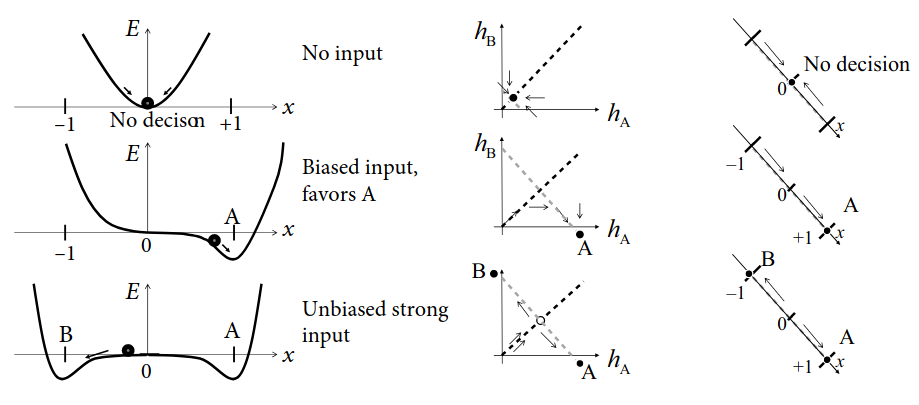
\includegraphics[width=0.95\textwidth,height=0.75\textheight]{competition4.png}
  \end{center}
\end{frame}

\begin{frame}{P4. Formal winner-take-all networks}

  Each outcome is represented by one population of excitatory neurons. We work with an effective inhibition of strength $\alpha > 0$ between the $K$ pools of neurons and with a self-interaction of strength $w_0$ within each pool of neurons.

  \begin{equation}
    \begin{aligned}
      A_k(t)&=g(h_k(t))\\
      \tau \frac{dh_k(t)}{dt}&=-h_k(t)+w_0g(h_k(t))-\alpha\sum_{j\neq k}w_{kj}g(h_j(t))+RI_k
    \end{aligned}
  \end{equation}

  Such networks are called \textbf{winner-take-all} networks, which are a standard topic of artificial neural networks.
  \footnote{\scalebox{0.8}{Hertz, J., Krogh, A., and Palmer, R. G.\textit{Introduction to the Theory of Neural Computation.} 1991 }}   
  \footnote{\scalebox{0.8}{Kohonen, T.\textit{Self-Organization and Associative Memory.} Springer-Verlag. 1984}}   
  \footnote{\scalebox{0.8}{Haykin, S.\textit{Neural Networks. Prentice} 1994}}   
\end{frame}

\begin{frame}{P4. Formal winner-take-all networks}
  Each artificial neuron receives an input $I_k$, has a positive feedback of magnitude $w_0$ onto itself but inhibits with strength $\alpha$ all other neurons.

  \begin{center}
    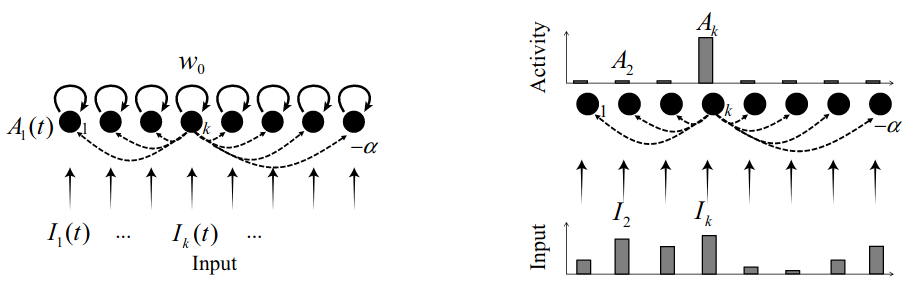
\includegraphics[width=0.8\textwidth,height=0.5\textheight]{winner.png}
  \end{center}

  Under fixed $I_k>0$, the network converges to a state where only a single “winner” neuron is active, i.e., \textbf{the one which receives the strongest input}.

\end{frame}

\begin{frame}{P4. Formal winner-take-all networks}

  We consider an arbitrary network of $K$ neuronal populations $1 \leq j \leq K$ with population rate $A_j = g(h_j) \geq 0$ where $g$ is a gain function with derivative $g' > 0$ and $h$ follows the dynamics

  $$\tau\frac{dh_j}{dt}=-h_j+RI_j+\sum\limits_k w_{jk}g(h_k)$$

  with fixed inputs $I_j$. If the coupling is symmetric, i.e., $w_{ij} = w_{ji}$, then the energy\footnote{\scalebox{0.8}{Cohen et.al.\textit{Absolute stability of global pattern formation and parallel memory storage by competitive neural networks.} 1983 }}   

  $$E=-\sum\limits_i\sum\limits_j w_{ij} A_i A_j-\sum\limits_i A_i RI_i+\sum\limits_i\int_{0}^{A_i}g^{-1}(a)da$$

  is \textbf{a Liapunov function} of the dynamics.
\end{frame}

\begin{frame}{P4. Formal winner-take-all networks}

  We exploit the fact that $w_{ij} = w_{ji}$ and $\frac{dA_i}{dt}=g'(h_i)\frac{dh_i}{dt}$ so as to find

  \begin{equation*}
    \begin{aligned}
      \frac{dE}{dt}&=-\sum\limits_i \left[\sum\limits_j w_{ij}A_j\right]g'(h_i)\frac{dh_i}{dt}-\sum\limits_i RI_ig'(h_i)\frac{dh_i}{dt}+\sum\limits_i g^{-1}(A_i)g'(h_i)\frac{dh_i}{dt}\\
      &=-\tau \sum\limits_i g'(h_i)\left[\frac{dh_i}{dt}\right]^2 \leq 0 \\
    \end{aligned}
  \end{equation*}

  Furthermore, since the neuronal gain function stays below a biologically sustainable firing rate $g(x) \leq A_{max}$, the energy is bounded from below.


\end{frame}


%-----------------------------------------------------------------------

\begin{frame}{Summary}
  \begin{itemize}
    \item 1. Decisions are prepared and \textbf{made in the brain} so that numerous physiological correlates of decision making can be found in the human and monkey cortex.
    \item 2. An influential computational \textbf{model} describes decision making \textbf{as the competition} of several populations of excitatory neurons which share a common pool of inhibitory neurons. 
    \item 3. Under suitable conditions, the explicit model of inhibitory neurons can be replaced by an effective \textbf{inhibitory coupling} between excitatory populations.
    \item 4. In a rate model, the competitive interactions between two excitatory populations can be understood using \textbf{phase plane analysis}.
    \item 5. Equivalently, the decision process can be described as downward motion in an energy landscape which plays the role of a \textbf{Liapunov function}.
  \end{itemize}
\end{frame}













%=======================================================================
\makebottom

\end{document}
